\documentclass[12pt]{article}

\usepackage[portuguese]{babel}

\usepackage{graphicx}
\usepackage[section]{placeins}
\usepackage{float}
\usepackage{url}

\graphicspath{ {figures} }

\author{João Vitor Maia Neves Cordeiro (19100532)}
\title{Bancos de dados multimídia: estudo teórico}
\date{\today}

\begin{document}

\maketitle

\begin{abstract}

Esse trabalho se propõe a introduzir e discutir de forma breve os conceitos básicos e tecnologias utilizadas para bancos de dados que trabalham com dados multimídia.
O primeiro foco foi no detalhamento dos conceitos iniciais, como a diferença entre dados multimídia e dados convencionais, após isso discutimos os potenciais requisitos que aplicações esperam de bancos de dados multimídia e por último apresentamos ferramentas utilizadas para trabalhar com esses tipos de dados.

\end{abstract}

\section{Introdução}

Desde antes da existência e difusão conexões rápidas o suficiente para que usuários conseguissem produzir, consumir e compartilhar conteúdo em imagem, áudio e vídeo através da internet, nós como sociedade já possuíamos maneiras de armazenar e indexar esse tipo de conteúdo de forma física em bibliotecas e cinematecas.

Esse tipo de esforço mostra como temos a necessidade de preservar história, memória e arte de forma acessível, e com os avanços em tecnologias de armazenamento, transmissão e processamento no começo do século 21, a computação ganhou um papel nessa área. Apesar de os principais bancos de dados atualmente trabalharem predominantemente com dados textuais, ainda existem dentro deles funcionalidades destinadas a auxiliar no armazenamento de conteúdo multimídia.

Além disso, existem ferramentas mais específicas para lidar apenas com esse tipo de estrutura, atualmente pouco difundidas, mas com um papel importante no início das discussões sobre o assunto na década passada.

\section{Dados multimídia}

Os primeiros SGBDs foram criados e comercializados na década de 60, as tecnologias de armazenamento e transmissão de dados na época eram ainda rudimentares se compararmos ao cenário atual, por isso esses sistemas proviam suporte apenas para um pequeno conjunto de tipos de dados, normalmente alfanuméricos. 
Mesmo com essas limitações impostas pela tecnologia, o conceito de SGBD foi um grande avanço da computação, pois permitia agora que administradores de sistemas mantessem uma base de dados centralizada e com uma certa consistência de escrita e leitura. 

Com a evolução desses sistemas, outros conceitos foram sendo criados e colocados a teste, entre eles o modelo relacional, que se provou uma outra grande revolução computacional devido ao seu formalismo baseado na álgebra relacional, que permitia termos muito mais corretude e segurança do que os modelos anteriores.
Entretanto, esse formalismo vem com um preço, SGBDs relacionais possuem uma grande dificuldade de trabalhar com representações complexas de dados, como campos multivalorados, dados temporais e o nosso estudo atual: dados multimídias.

Em um SGBD comum, existem regras a serem respeitadas para criar uma consulta, além de otimizações que podem ser pensadas em cima da consulta, tendo um formato geral que segue: quais objetos serão buscados, a quais tabelas esses objetos pertencem e qual o predicado será utilizado para determinar quais linhas serão retornadas.
Ao tentar aplicar esse mesmo modelo para dados multimídias, encontramos uma série de problemas relacionados a própria natureza desse tipo de dados:

\begin{itemize}
    \item Estrutura: ao contrário de dados alfanuméricos, os dados multimídia não costumam possuir uma estrutura rígida a ser seguida, o que dificulta buscas por conteúdo e indexação.
    \item Temporalidade e espacialidade: em dados multimídia é comum termos variáveis temporais, isso acontece principalmente em áudio e vídeo, onde o conteúdo a ser armazenado, processado e apresentado obedece uma certa sequência, fazendo com que os processos ordinários de SGBDs para essas operações não sejam aplicáveis a esse tipo de dados
    \item Volume de dados: o dados multimídia possuem um espaço em disco elevado, e cada vez mais esse tamanho vem crescendo devido a resolução de vídeos, imagens e áudios que melhoram conforme as tecnologias de captação avançam.
    \item Compressão: é muito comum a compressão de dados multimídia justamente para contornar o item citado acima, SGBDs precisariam implementar as diferentes maneiras de compressão utilizadas por esses tipos de dados para poderem conversar com outras aplicações de captação, edição e apresentação de dados multimídia.
\end{itemize}

Ainda contextualizando o cenário de trabalharmos com dados multimídia, não podemos deixar de citar que para cada uma das problemáticas já citadas, ainda existirão particularidades relacionadas ao tipo de dado multimídia utilizado e mais além, ao seu formato. 
Um problema que pode ser facilmente resolvível para áudios, pode não ser tão simples de resolver quando tratamos de vídeos. E mesmo um problema facilmente resolvível em áudios no formato AAC, pode vir a ser uma dificuldade ao se trabalhar com áudio no formato MP3.

\section{Bancos de dados multimídia}

Com o crescimento do uso de SGBDs, surge a necessidade de que esses sistemas possuam suporte para tipos mais complexos de dados, entre eles os dados multimídia. Desde então, estudos a cerca de SGBDMM (Sistemas gerenciadores de bancos de dados multimídia) começaram a ser conduzidos, com o objetivo de que o desenvolvimento desses sistemas pudesse alcançar o ponto onde eles nos forneceriam as mesmas facilidades que SGBDs fornecem para aplicações de dados convencionais.

Os primeiros estudos partiram direto do modelo relacional ou do modelo relacional estendido, esperando que as técnicas utilizadas nesses 2 modelos fossem o suficiente para lidar com indexação, buscas, gerenciamento de memória, concorrência, integridade de dados e outros problemas já solucionados por SGBDs. Isso acabou se provando um equívoco, já que pela diferença de natureza entre os tipos de dados trabalhados, as mesmas técnicas não puderam ser aplicadas em SGBDMMs e resultaram em falhas nesses projetos.

Ainda haviam novos requisitos surgindo diariamente para bancos multimídia, como a busca por subimagens dentro de imagens em um banco, busca de trechos de músicas em uma grande coleção de músicas para identificar possíveis plágios ou samples.

\section{Aplicações possíveis para bancos de dados multimídia}

Assim como no caso dos bancos de dados relacionais tradicionais, os bancos multimídia possuem aplicações que ultrapassam os limites apenas da área de computação, podendo ser aproveitados por diversas outras áreas que tenham a necessidade de armazenamento, processamento e indexação de algum tipo de dados multimídia.
Podemos incluir casos como a área da educação, que seria beneficiada com um melhor gerenciamento de conteúdo digital atráves de técnicas de indexação e busca, a área da saúde que já vem avançando bastante seus usos de tecnologias como visão computacional, poderia aderir a bancos de imagens médicas relacionadas a diagnósticos e tratamentos. A área de entretenimento também já evoluiu com tecnologias que permitem hoje streaming de vídeos, mas poderia crescer ainda mais com a disponibilização de técnicas novas para processamento de dados multimídia dentro de seus próprios catálogos.

A própria comunidade científica como um todo possui grande interesse no desenvolvimento dessas tecnologias que poderiam facilitar a colaboração entre pesquisadores do mundo todo, alimentando bases de dados com material científico, estudos públicos e conteúdo gratuito de divulgação científica disponibilzado para o mundo todo em questão de segundos. Além de facilitar no desenvolvimento de novas pesquisas utilizando as técnicas de busca dentro de mídias já existentes.

\section{Arquitetura de um SGBDMM}

Já vimos que existem diferenças significativas entre os dados convencionais e dados multimídia, mas ainda é necessário entender as possíveis diferenças entre SGBDs e SGBDMMs. Uma das principais diferenças é que ao utilizarmos técnicas de busca em imagens ou vídeos, até as técnicas mais avançadas atualmente irão retornar uma resposta baseada em um grau de similaridade, ou seja, o nível de confiança nessa resposta apesar de ser alto, ainda não é completo. Além disso, essas consultas exigem modelos que são consideravelmente mais complexos do que as buscas em dados convencionais e podem acarretar em uma demora com a qual o usuário ainda não está acostumado \cite{bittencourt}.

\cite{biazi} organiza o SGBDMM de 3 formas diferentes, a partir de princípios estabelecidos para auxiliar o entendimento e aplicação dessa arquitetura.

\subsection{Princípio da autonomia}

Nesta organização, cada tipo de mídia possui um motor próprio, com algoritmos dedicados e otimizados apenas para o determinado tipo. Dessa forma ao receber uma consulta, antes de começar o processamento em si, o SGBDMM utiliza técnicas internas para definir quais serão os tipos de mídias a serem explorados naquela consulta, e repassa a requisição de consulta para esses motores específicos.

\begin{figure}[H]
    \centering
    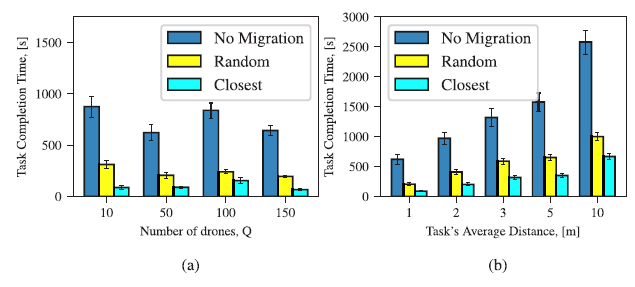
\includegraphics[width=0.7\linewidth]{figure_1.png}
    \caption{Princípio de autonomia. Retirado de CUNHA\cite{cunha}}
\end{figure}

\subsection{Princípio da uniformidade}

Neste caso temos um único motor de pesquisa com um índice único também, as consultas são realizadas a partir de metadados enviados ao motor de busca, que consulta o índice a partir dos metadados para encontrar resultados. Apesar de ser uma arquitetura simples de implementar e que traz resultados rápidos, os objetos guardados no banco precisam de metadados relacionados a eles que devem ser preenchidos de forma manual ou automática, e a corretude da busca é dependente dessas anotações realizadas em cima dos objetos.

\begin{figure}[H]
    \centering
    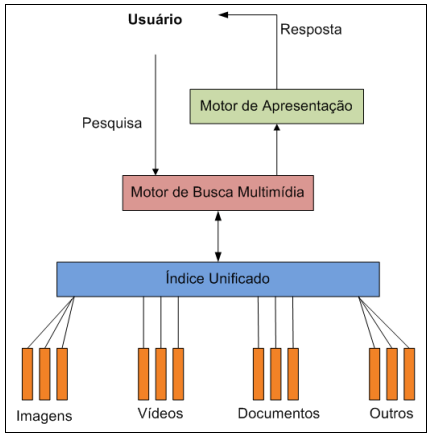
\includegraphics[width=0.7\linewidth]{figure_2.png}
    \caption{Princípio de uniformidade. Retirado de CUNHA\cite{cunha}}
\end{figure}

\subsection{Princípio de organização híbrida}

O último dos princípios une os pontos fortes dos dois últimos princípios, dessa forma pode-se adaptar cada princípio anterior para um tipo de mídia, utilizando busca por metadados para tipos de mídias que podem ser mais facilmente anotados de forma automática, e a busca com algoritmos específicos para mídias que não possuam essa facilidade. Essa organização possui uma complexidade maior de implementação devido à necessidade de implementar as duas últimas e ainda um controle acima disso decidindo qual método utilizar para uma determinada consulta.

\begin{figure}[H]
    \centering
    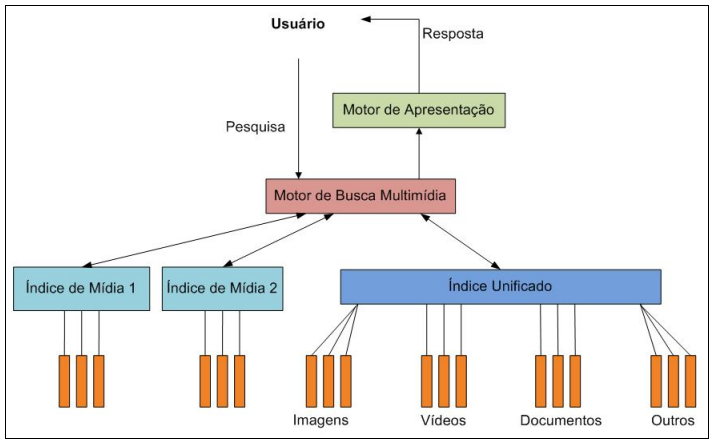
\includegraphics[width=0.7\linewidth]{figure_3.png}
    \caption{Princípio de organização híbrida. Retirado de CUNHA\cite{cunha}}
\end{figure}

\nocite{*}
\medskip

\bibliographystyle{ieeetr}
\bibliography{biblio}

\end{document}